% Homework #4
% COSC552 HCI
%
% Byron Heads
% E00062946

\documentclass[12pt]{report}

\usepackage{graphics}
\usepackage{hyperref}

\title{Homework Set 4 \\
    COSC552 HCI}
\author{ Byron Heads \\
    E00062946 }
\date{\today}

\begin{document}
\maketitle

\chapter*{A}
The icons used are the open source Silk Icons from 
\url{http://www.famfamfam.com/}.  The interface was created with 
wxFormBuilder (\url{http://wxformbuilder.org/}) using the wxWidgets
(\url{http://www.wxwidgets.org/}) library in C++. 

\begin{figure}[h!]
\center{\resizebox{280pt}{!}{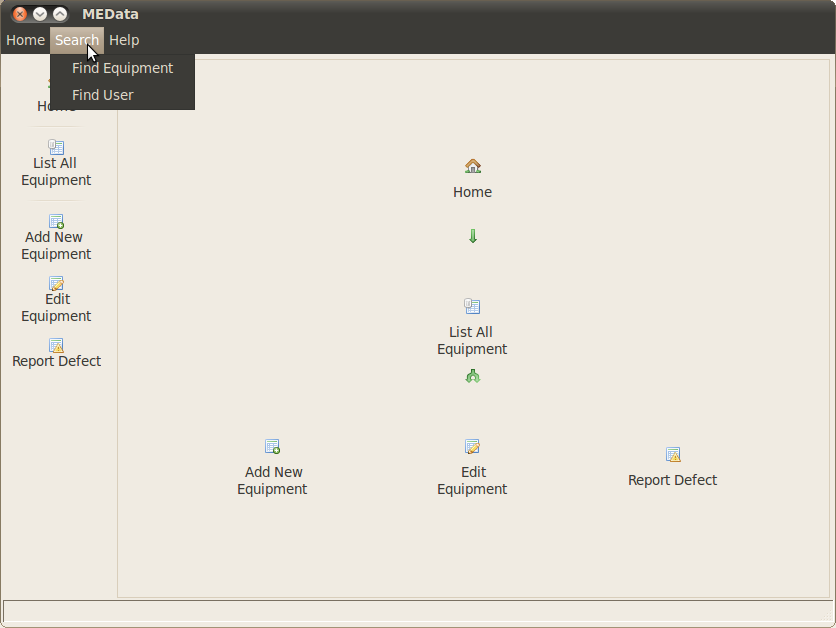
\includegraphics{ss1.png}}}
\caption{The main programs menu screen showing the home screen.  Selecting
a menu item will change the panel to that screen.}
\end{figure}


\begin{figure}[h!]
\center{\resizebox{280pt}{!}{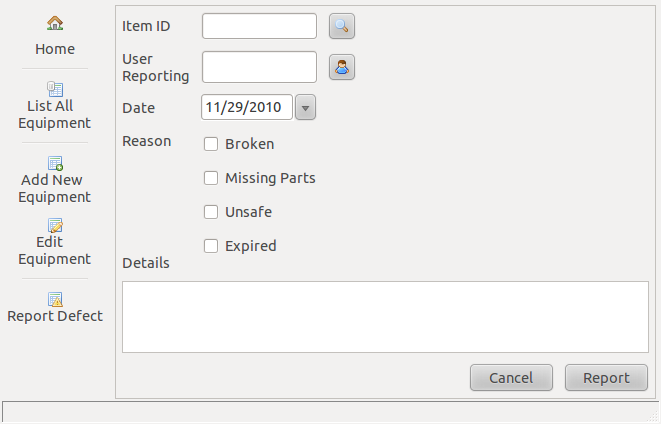
\includegraphics{ss2.png}}}
\caption{Here the user can input a defective item into the system.  The
user can look up the part number from the item lookup dialog.  The user
can also do a look up on there user name and select the date from the 
date picker.  The user name is default to the user logged in.  The date is
defaulted to current date.  The reason for the defect can be selected, 
and the user can enter more details if needed.}
\end{figure}

\begin{figure}[h!]
\center{\resizebox{280pt}{!}{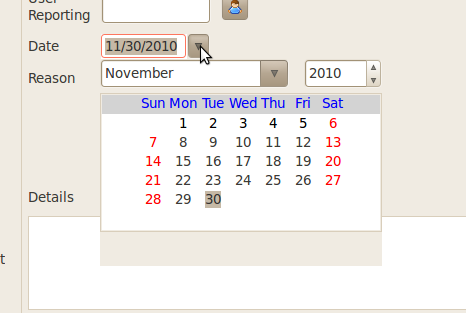
\includegraphics{ss3.png}}}
\caption{The date picker in action.}
\end{figure}

\begin{figure}[h!]
\center{\resizebox{250pt}{!}{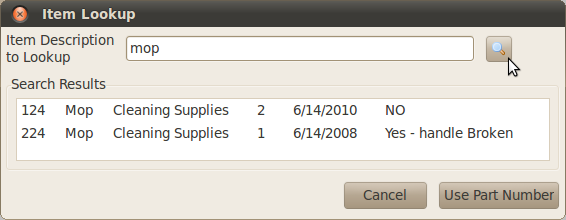
\includegraphics{ss4.png}}}
\caption{The item lookup window is used to help search for a part number
in the equipment database.  The users enters a search term to search for.
If any results are found they are displayed in the results window.  The
user can select an item and click the Use Part Number button.  The part
number will be entered into the correct field.}
\end{figure}

\pagebreak
\chapter*{B}

\begin{figure}[h!]
\center{\resizebox{280pt}{!}{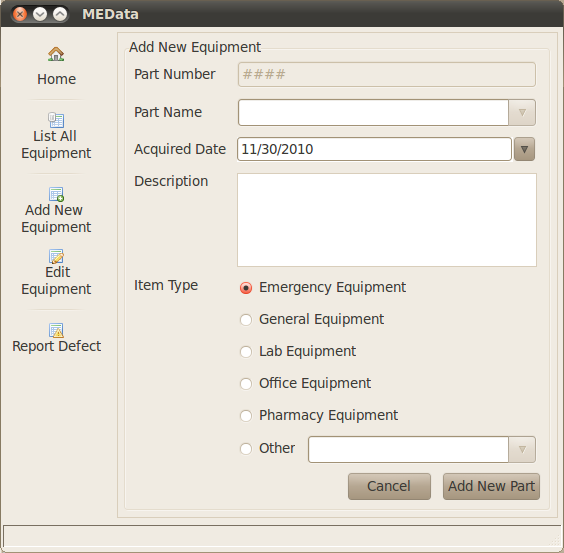
\includegraphics{ss5.png}}}
\caption{This window allows the user to add a new piece of equipment into
the database.  The part number is generated automatically for the user.  
The user enters a part name, or can select for the drop down one of the 
most common part names.  The user enters the acquired date of the item, and
input more details about the part.  Last the user selects an item category
for the part.  They can also use other and enter a new category. }
\end{figure}

\begin{figure}[h!]
\center{\resizebox{280pt}{!}{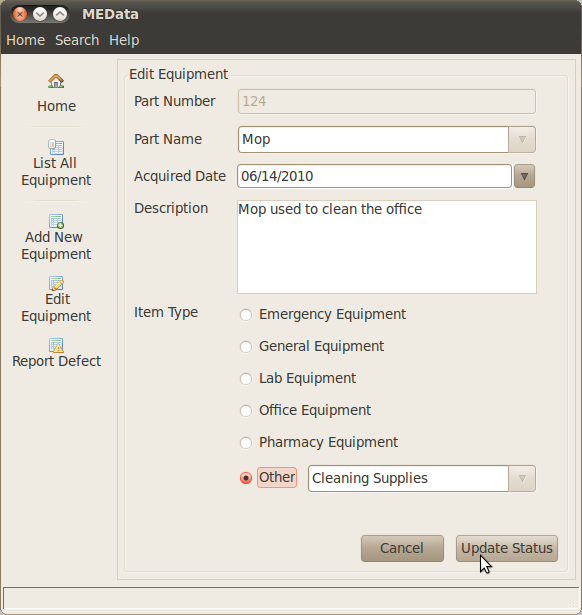
\includegraphics{ss6.png}}}
\caption{The edit equipment screen is the same as the Add New Equipment
screen.  This makes it easier for users to learn how to handle equipment.}
\end{figure}

\begin{figure}[h!]
\center{\resizebox{280pt}{!}{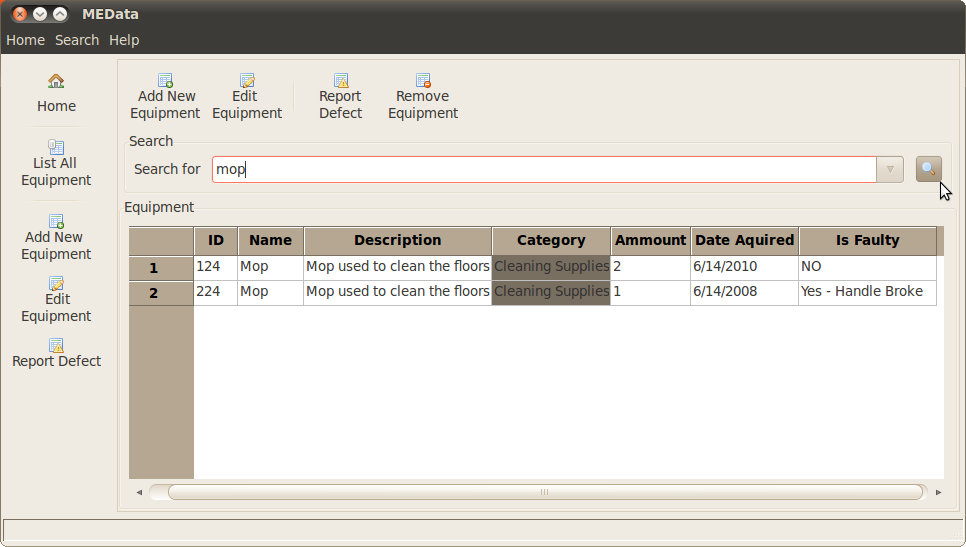
\includegraphics{ss7.png}}}
\caption{ This screen lists all of the equipment in the database.  Table
drawing was not working at this time.  With this screen the user can 
add, edit, report a defect, or remove a part from the database.  The user
can search and sort the database as needed.}
\end{figure}


\chapter*{C}

MEData is a medical inventory database system.  It is used to track your
clinic's inventory.  The program starts at the home screen.  The home screen
reflects the choices you can make on the sidebar.  You can start by 
clicking on the List All Equipment button.  The main panel will change to 
the equipment list screen.  From here you can see everything thats in the
database.  You can add new parts, edit a part, report a part as defective,
or remove a part from the database.  You can also run searches on parts, or
sort the parts list.

Help for this program would include inline help, when the user enters
invalid data into a field to will be marked, and the user will have to
correct the data before they can move on.  Help will also be available 
from in program help menu.  Which is currently not in the demo images.

\end{document}

